\documentclass[aspectratio=43]{beamer}
\usepackage{graphicx}

\usepackage{amsmath}
\usepackage{amsfonts}
\usepackage{amssymb}
\usepackage{amsthm}
\usepackage{tikz}
\usepackage{xcolor}
\usepackage{array}
\usepackage{enumitem}
\usepackage{tabularx}

\usetheme{Madrid}
\usecolortheme{default}

\setbeamertemplate{navigation symbols}{}

\setbeamertemplate{footline}{}

\title{}
\author{}
\date{}

\begin{document}
\begin{frame}
\frametitle{Linear recurrences: motivating example}

\begin{block}{Problem}
Solve the \textcolor{blue}{linear recurrence}
\[h_n = 5h_{n-1} - 6h_{n-2} \quad (n \geq 2)\]
with the initial conditions $h_0 = 1$ and $h_1 = -2$.
\end{block}

\begin{block}{Solution}
\begin{align*}
\sum_{n \geq 2} h_n x^n &= 5 \sum_{n \geq 2} h_{n-1}x^n - 6 \sum_{n \geq 2} h_{n-2}x^n \\
&= 5x \sum_{n \geq 2} h_{n-1}x^{n-1} - 6x^2 \sum_{n \geq 2} h_{n-2}x^{n-2} \\
&= 5x \sum_{n \geq 1} h_n x^n - 6x^2 \sum_{n \geq 0} h_n x^n \\
h(x) - h_1x - h_0 &= 5x(h(x) - h_0) - 6x^2 h(x)
\end{align*}
\end{block}

\end{frame}

\begin{frame}
    \begin{center}
        Math 465: Introduction to Combinatorics
        
        \vspace{1cm}
        
        Andrew Sack
        
        \vspace{1cm}
        
        \hrulefill
        
        \vspace{0.5cm}
        
        Homework \#3 will be due Monday evening.
        
        \vspace{0.5cm}
        
        \hrulefill
        
        \vspace{0.5cm}
        
        These slides will be posted on Canvas.
    \end{center}
\end{frame}

\begin{frame}
\frametitle{Linear recurrences: the generating functions approach}

\begin{block}{Problem}
Solve the recurrence relation
\[
h_n = 5h_{n-1} - 6h_{n-2}
\]
with the initial conditions $h_0 = 1$ and $h_1 = -2$.
\end{block}

\begin{block}{Solution (continued)}
\begin{align*}
h(x) - h_1 x - h_0 &= 5x(h(x) - h_0) - 6x^2 h(x) \\
h(x) + 2x - 1 &= 5x(h(x) - 1) - 6x^2 h(x) \\
h(x) &= \frac{1-7x}{1 - 5x + 6x^2} = \frac{1-7x}{(1-2x)(1-3x)} = \frac{5}{1-2x} - \frac{4}{1-3x} \\
h(x) &= 5(1 + 2x + 4x^2 + 8x^3 + \dots) - 4(1 + 3x + 9x^2 + 27x^3 + \dots) \\
h_n &= 5 \cdot 2^n - 4 \cdot 3^n \leftarrow \text{linear combination of geometric progressions}
\end{align*}

While this approach can be developed systematically, we won't do it.
\end{block}

\end{frame}

\begin{frame}
\frametitle{Linear recurrences: general set-up}

We aim to solve \textbf{linear recurrences with constant coefficients}, i.e., recurrences of the form
\begin{equation*}
    (*) \qquad h_n + a_1h_{n-1} + a_2h_{n-2} + \cdots + a_kh_{n-k} = 0.
\end{equation*}
Here
\begin{itemize}
    \item $k$ is the \textbf{order} of the recurrence;
    \item $a_1, \dots, a_k$ are its \textbf{coefficients};
    \item $a_k \neq 0$ without loss of generality;
    \item the $k$ \textbf{initial values} $h_0, h_1, \dots, h_{k-1}$ are given;
    \item $n$ takes values $k, k+1, k+2, \dots$.
\end{itemize}

\bigskip

\begin{block}{Example}
    \begin{equation*}
        h_n - 5h_{n-1} + 6h_{n-2} = 0
    \end{equation*}
\end{block}

\bigskip

The theory of linear recurrences is very similar to the theory of linear differential equations.

\end{frame}

\begin{frame}
\frametitle{General solution in the case of distinct roots}

\begin{itemize}
    \item[(*)] $h_n + a_1h_{n-1} + a_2h_{n-2} + \cdots + a_kh_{n-k} = 0$
\end{itemize}

\begin{itemize}
    \item[\textbf{Three Lemmas}]
    \begin{itemize}
        \item The solutions of (*) form a vector space of dimension $k$.
        \item A geometric progression $h_n = q^n$ satisfies (*) if and only if
        \begin{itemize}
            \item[ (**)] $q^k + a_1q^{k-1} + a_2q^{k-2} + \cdots + a_k = 0$.
        \end{itemize}
        \item Geometric progressions with distinct ratios are linearly independent.
    \end{itemize}
\end{itemize}

These lemmas imply the following theorem.

\begin{itemize}
    \item[\textbf{Theorem}]
    If the characteristic equation (**) has distinct roots $q_1, \dots, q_k$, then
    \begin{center}
        $h_n = \sum_{i=1}^k c_i q_i^n$
    \end{center}
    is the general solution of (*).
\end{itemize}

\end{frame}

\begin{frame}
\frametitle{Geometric progressions}

\begin{block}{Lemma}
Geometric progressions with distinct ratios are linearly independent.
\end{block}

\begin{block}{Proof [sketch]}
Suppose that $k$ geometric progressions (in the example below, $k = 3$)
\begin{align*}
& 1 \quad q \quad q^2 \quad \dots \\
& 1 \quad r \quad r^2 \quad \dots \\
& 1 \quad s \quad s^2 \quad \dots
\end{align*}
(with $q, r, s$ distinct and nonzero) are linearly dependent. Then
\[
\det \begin{pmatrix}
1 & q & q^2 \\
1 & r & r^2 \\
1 & s & s^2
\end{pmatrix} = 0 \implies \exists (a, b, c) \neq (0, 0, 0)
\begin{cases}
a + bq + cq^2 = 0, \\
a + br + cr^2 = 0, \\
a + bs + cs^2 = 0.
\end{cases}
\]
Thus $a + bt + ct^2$, a nonzero polynomial of degree $\leq k - 1$,
has $k$ distinct roots, a contradiction.
\end{block}

\end{frame}

\begin{frame}
\frametitle{The characteristic equation}

\begin{itemize}
    \item [(*)] $h_n + a_1h_{n-1} + a_2h_{n-2} + \dots + a_kh_{n-k} = 0$
\end{itemize}

\begin{itemize}
    \item [\textbf{Lemma}]
    \item For $q \neq 0$, the geometric progression $h_n = q^n$ satisfies (*) if and only if
    \item [(**)] $q^k + a_1q^{k-1} + a_2q^{k-2} + \dots + a_k = 0$.
\end{itemize}

\begin{itemize}
    \item [\textbf{Proof}]
    \item \begin{align*}
         q^n + a_1q^{n-1} + a_2q^{n-2} + \dots + a_kq^{n-k} &= 0 \\
         \Leftrightarrow q^k + a_1q^{k-1} + a_2q^{k-2} + \dots + a_k &= 0
    \end{align*}
\end{itemize}

Equation (**) is the \textcolor{blue}{characteristic equation} for the recurrence (*).

\begin{itemize}
    \item [\textbf{Example}]
    \item [(*)] $h_n - 5h_{n-1} + 6h_{n-2} = 0$
    \item [(**)] $q^2 - 5q + 6 = 0$
    \item Roots: $q=2$ and $q=3$. Solutions $h_n = 2^n$ and $h_n = 3^n$.
\end{itemize}

\end{frame}

\begin{frame}
\frametitle{The vector space of solutions of a linear recurrence}

\begin{block}{Lemma}
The solutions of a linear recurrence
\begin{align*}
    (*) \qquad h_n + a_1 h_{n-1} + a_2 h_{n-2} + \cdots + a_k h_{n-k} = 0
\end{align*}
form a vector space. The dimension of this vector space is $k$.
\end{block}

\begin{block}{Example}
\begin{align*}
    (*) \qquad h_n - 5h_{n-1} + 6h_{n-2} = 0
\end{align*}

\begin{tabular}{cccccc}
    $1$ & $0$ & $-6$ & $-30$ & $-114$ & $\cdots$ \\
    $0$ & $1$ & $5$ & $19$ & $65$ & $\cdots$ \\
    $a$ & $b$ & $-6a+5b$ & $-30a+19b$ & $-114a+65b$ & $\cdots$
\end{tabular}
\end{block}

\begin{block}{proof}
We can freely choose the first n entries in a sequence. The rest are determined.
\end{block}

\end{frame}

\begin{frame}
\frametitle{Domino tilings}

\begin{block}{Theorem}
The number of ways to tile a $2 \times n$ rectangular board by dominoes is equal to the Fibonacci number $f_{n+1}$.
\end{block}

\begin{itemize}
    \item $\emptyset$
    \item \begin{tikzpicture}[scale=0.3]
    \draw (0,0) rectangle (1,2);
    \end{tikzpicture}
    \item 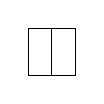
\begin{tikzpicture}[scale=0.3]
    \draw (0,0) rectangle (1,2);
    \draw (1,0) rectangle (2,2);
    \end{tikzpicture}
    \item 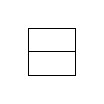
\begin{tikzpicture}[scale=0.3]
    \draw (0,0) rectangle (2,1);
    \draw (0,1) rectangle (2,2);
    \end{tikzpicture}
    \item 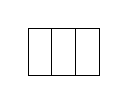
\begin{tikzpicture}[scale=0.3]
    \draw (0,0) rectangle (1,2);
    \draw (1,0) rectangle (2,2);
    \draw (2,0) rectangle (3,2);
    \end{tikzpicture}
    \item 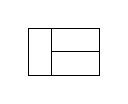
\begin{tikzpicture}[scale=0.3]
    \draw (0,0) rectangle (1,2);
    \draw (1,0) rectangle (3,1);
    \draw (1,1) rectangle (3,2);
    \end{tikzpicture}
    \item 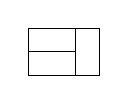
\begin{tikzpicture}[scale=0.3]
    \draw (0,0) rectangle (2,1);
    \draw (0,1) rectangle (2,2);
    \draw (2,0) rectangle (3,2);
    \end{tikzpicture}
    \item 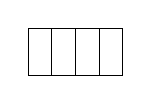
\begin{tikzpicture}[scale=0.3]
    \draw (0,0) rectangle (1,2);
    \draw (1,0) rectangle (2,2);
    \draw (2,0) rectangle (3,2);
    \draw (3,0) rectangle (4,2);
    \end{tikzpicture}
    \item 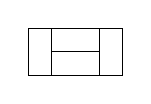
\begin{tikzpicture}[scale=0.3]
    \draw (0,0) rectangle (1,2);
    \draw (1,0) rectangle (3,1);
    \draw (1,1) rectangle (3,2);
    \draw (3,0) rectangle (4,2);
    \end{tikzpicture}
    \item 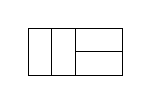
\begin{tikzpicture}[scale=0.3]
    \draw (0,0) rectangle (1,2);
    \draw (1,0) rectangle (2,2);
    \draw (2,0) rectangle (4,1);
    \draw (2,1) rectangle (4,2);
    \end{tikzpicture}
    \item 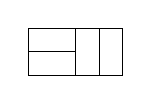
\begin{tikzpicture}[scale=0.3]
    \draw (0,0) rectangle (2,1);
    \draw (0,1) rectangle (2,2);
    \draw (2,0) rectangle (3,2);
    \draw (3,0) rectangle (4,2);
    \end{tikzpicture}
    \item 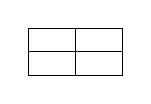
\begin{tikzpicture}[scale=0.3]
    \draw (0,0) rectangle (2,1);
    \draw (0,1) rectangle (2,2);
    \draw (2,0) rectangle (4,1);
    \draw (2,1) rectangle (4,2);
    \end{tikzpicture}
    \item 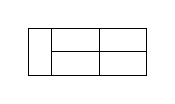
\begin{tikzpicture}[scale=0.3]
    \draw (0,0) rectangle (1,2);
    \draw (1,0) rectangle (3,1);
    \draw (1,1) rectangle (3,2);
    \draw (3,0) rectangle (5,1);
    \draw (3,1) rectangle (5,2);
    \end{tikzpicture}
    \item 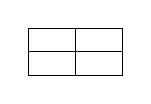
\begin{tikzpicture}[scale=0.3]
    \draw (0,0) rectangle (2,1);
    \draw (0,1) rectangle (2,2);
    \draw (2,0) rectangle (4,1);
    \draw (2,1) rectangle (4,2);
    \end{tikzpicture}
\end{itemize}

\end{frame}

\begin{frame}
\frametitle{Binary strings with no consecutive 1's}

\begin{block}{Theorem}
The number of binary strings of length $n$ that do not contain a pair of consecutive 1's is equal to the Fibonacci number $f_{n+2}$.
\end{block}

\begin{center}
$\emptyset$ \quad
0 \quad
00 \quad
000 \quad
0000 \\
1 \quad
01 \quad
001 \quad
0001 \\
\quad
10 \quad
010 \quad
0010 \\
\quad
\quad
100 \quad
0100 \\
\quad
\quad
101 \quad
0101 \\
\quad
\quad
\quad
1000 \\
\quad
\quad
\quad
1001 \\
\quad
\quad
\quad
1010
\end{center}

\end{frame}

\begin{frame}
\frametitle{Sums of 1's and 2's}

\begin{block}{Theorem}
The number of ways to represent $n$ as an ordered sum of summands each of which is equal to 1 or 2 is equal to the Fibonacci number $f_{n+1}$.
\end{block}

\bigskip

\begin{tabular}{lllll}
$\emptyset$ & 1 & 1+1 & 1+1+1 & 1+1+1+1 \\
& & 2 & 1+2 & 1+1+2 \\
& & & 2+1 & 1+2+1 \\
& & & & 2+1+1 \\
& & & & 2+2 \\
& & & & \\
\end{tabular}

\bigskip

\begin{tabular}{l}
1+1+1+1+1 \\
1+1+1+2 \\
1+1+2+1 \\
1+2+1+1 \\
1+2+2 \\
2+1+1+1 \\
2+1+2 \\
2+2+1 \\
\end{tabular}

\end{frame}

\begin{frame}
\frametitle{Formula for the Fibonacci numbers}
\begin{block}{Theorem}
\[f_n = \frac{1}{\sqrt{5}} \left( \frac{1 + \sqrt{5}}{2} \right)^n - \frac{1}{\sqrt{5}} \left( \frac{1 - \sqrt{5}}{2} \right)^n.\]
\end{block}

\begin{block}{Corollary}
The Fibonacci number $f_n$ is the closest integer to $\frac{1}{\sqrt{5}} \left( \frac{1 + \sqrt{5}}{2} \right)^n$.
\end{block}

\begin{block}{Corollary}
\[\lim_{n \to \infty} \frac{f_{n+1}}{f_n} = \frac{1 + \sqrt{5}}{2}.\]
\end{block}

\end{frame}

\begin{frame}
\frametitle{Fibonacci numbers and square tilings}

\begin{tikzpicture}
\draw (0,0) rectangle (13,8);

\draw (0,3) rectangle (5,8);
\node at (2.5,5.5) {\color{red} 8};

\draw (5,0) rectangle (13,8);
\node at (9,4) {\color{red} 13};

\draw (0,0) rectangle (5,3);
\node at (2.5,1.5) {\color{red} 5};

\draw (5,0) rectangle (3,3);
\node at (6.5,1.5) {\color{red} 3};

\draw (5,2) rectangle (6,3);
\node at (5.5,2.5) {\color{red} 2};

\fill[gray] (5,2) rectangle (6,3);
\node at (4.5,2.5) {\color{red} 1};

\end{tikzpicture}

\end{frame}

\usepackage{graphicx}

\begin{frame}
\frametitle{Phyllotaxis}

\begin{columns}
    \begin{column}{0.24\textwidth}
        \includegraphics[width=\linewidth]{example-image-a}
        \centering
        8 parallel rows of\\
        scales spiralling\\
        gradually
    \end{column}
    \begin{column}{0.24\textwidth}
        \includegraphics[width=\linewidth]{example-image-a}
        \centering
        13 parallel rows of\\
        scales spiralling at a\\
        medium slope
    \end{column}
    \begin{column}{0.24\textwidth}
        \includegraphics[width=\linewidth]{example-image-a}
        \centering
        21 parallel rows of\\
        scales spiralling at a\\
        steep slope
    \end{column}
    \begin{column}{0.24\textwidth}
        \includegraphics[width=\linewidth]{example-image-a}
        \centering
        21 parallel rows of\\
        scales spiralling at a\\
        steep slope
    \end{column}
\end{columns}

\end{frame}

\begin{frame}
\frametitle{Towards the formula for the Fibonacci numbers}

The Fibonacci recurrence
\[
f_n = f_{n-1} + f_{n-2}
\]
has the characteristic equation
\[
q^2 - q - 1 = 0.
\]
The roots of this equation are
\[
q_1 = \frac{1 + \sqrt{5}}{2}, \quad q_2 = \frac{1 - \sqrt{5}}{2}.
\]
Consequently,
\[
f_n = c_1 q_1^n + c_2 q_2^n,
\]
for some constants $c_1$ and $c_2$. To find $c_1$ and $c_2$, we write
\[
f_0 = 0 = c_1 + c_2,
\]
\[
f_1 = 1 = c_1 q_1 + c_2 q_2 = c_1(q_1 - q_2) = c_1 \sqrt{5}.
\]
Thus $c_1 = \frac{1}{\sqrt{5}}$ and $c_2 = -\frac{1}{\sqrt{5}}$.

\end{frame}

\begin{frame}
\frametitle{Spirals in a cactus}

\begin{center}
\includegraphics[width=0.8\textwidth]{placeholder}
\end{center}

\begin{center}
21 and 34 spirals
\end{center}

\end{frame}

\begin{frame}
\frametitle{The case of distinct roots: example}

\begin{block}{Theorem}
Given a linear recurrence
\begin{equation*}
(*) \qquad h_n + a_1h_{n-1} + a_2h_{n-2} + \dots + a_kh_{n-k} = 0,
\end{equation*}
if the characteristic equation
\begin{equation*}
q^k + a_1q^{k-1} + a_2q^{k-2} + \dots + a_k = 0
\end{equation*}
has distinct roots $q_1, \dots, q_k$, then the general solution of (*) is given by
\begin{equation*}
h_n = \sum_{i=1}^k c_i q_i^n.
\end{equation*}
\end{block}

\begin{block}{Example}
The general solution of the recurrence $h_n - 5h_{n-1} + 6h_{n-2} = 0$ is given by $h_n = c_1 \cdot 2^n + c_2 \cdot 3^n$. For the initial conditions $h_0 = 1$ and $h_1 = -2$, we get $c_1 + c_2 = 1$ and $2c_1 + 3c_2 = -2$, implying $c_1 = 5$ and $c_2 = -4$.
\end{block}

\end{frame}

\begin{frame}
Fibonacci numbers

\vspace{0.5cm}
\centering
\setlength{\fboxsep}{8pt}
\colorbox{lightgray}{
\begin{minipage}{0.9\textwidth}
Definition [Pingala, \textit{ca.} 200 BCE; Leonardo di Pisa, 1202]
\end{minipage}}

\vspace{0.2cm}
The \textbf{Fibonacci numbers} are defined by the recurrence
\[ f_n = f_{n-1} + f_{n-2} \quad (n \geq 2) \]
together with the initial conditions $f_0 = 0, f_1 = 1$.

\vspace{0.5cm}

\begin{tabular}{|c|c|c|c|c|c|c|c|c|c|c|c|c|c|c|}
\hline
$n$ & 0 & 1 & 2 & 3 & 4 & 5 & 6 & 7 & 8 & 9 & 10 & 11 & 12 & 13 & 14 \\ \hline
$f_n$ & 0 & 1 & 1 & 2 & 3 & 5 & 8 & 13 & 21 & 34 & 55 & 89 & 144 & 233 & 377 \\ \hline
\end{tabular}

\end{frame}
\end{document}